\chapter{Pilot Study}
\label{ch:Pilot}

I employed the case study research strategy \cite{Yin:03} to empirically study Zorro's TDD development behaviors inference. In order to validate Zorro, I conducted a pilot study at the University of Hawaii in Fall 2005. This study shows that the participant observation research method using ESR is an acceptable research method for Zorro validation and it also shows that Zorro can accurately recognize development behaviors of TDD in a simple project development setting.

\section{Purpose of the Study}
The pilot study served as a dry-run test to the chosen case study research strategy. As mentioned in Chapter \ref{ch:Research}, the purpose of the pilot study was to test ESR, as well as to validate Zorro's data collection and behaviors inference of TDD.

\section{Research Questions}
\label{sec:Pilot-Questions}

The specific research questions for the pilot study were:
\begin{itemize}
 \item Q1a: Is ESR a suitable tool for Zorro validation study?
 \item Q1b: Does Zorro collect enough low-level development activities to
   infer developer's TDD behaviors?
 \item Q1c: Does Zorro's inference of TDD agree with analyses based upon
   participant observation?
\end{itemize}

Note that these specific research questions corresponded to the main research questions Q1: \textit{Can Zorro automate the recognition of TDD behaviors using automatically collected software metrics?}

\section{Experiment Design}
\label{sec:Pilot-Design}
The pilot study was largely a one-shot case study in which participants were exposed to TDD. Creswell \cite{Creswell:03} suggests the following notation for it:
  \begin{tabular}{p{0.5cm}lp{1cm}l} 
    & Group A  & & X ------ O
  \end{tabular}

where group A represents a group of participants, X represents an exposure of a group to an experimental variable or event, and O represents an observation or measurement on an instrument. In this study, TDD was the treatment and Zorro was the instrument.  

\subsection{Participants}

In this study, I recruited seven experienced Java developers who were 
familiar with unit testing. 

\subsection{Materials}
The programming problem was the stack data structure. I gave the developers user stories which described the activities they were to perform in order to implement the stack.. Eclipse was the development tool. In addition, I also provided Doshi's TDD Rhythm \cite{TDDRhythm} and TDD Quick Reference Guide \cite{TDDQuickReference} as supporting materials. In order to improve participants' commitment to TDD, a To-Do list was supplied as the reference. 

\subsection{Instrument}
I instrumented participants' TDD development processes with the Hackystat Eclipse sensor and ESR. Participants were required to install the Hackystat Eclipse sensor and send the collected development activities to a remote Hackystat server. They also installed ESR which recorded their Eclipse windows as they participated in this study. 

\subsection{Procedure}
Since the pilot study configuration was very simple, participants were given the option to either work on a lab computer or on their own computers at home. For those who opted to work at home, I provided detailed step-by-step instructions to them.  

\begin{enumerate}
\item{Setup} 

Prior to the study I confirmed that the lab computer had the following software installed: 
  \begin{itemize}
    \item JDK 
    \item Eclipse IDE 
    \item Hackystat Eclipse Sensor \cite{HackystatSensorInstallation:06}
    \item Eclipse Screen Recorder \cite{esr}
  \end{itemize}
When participants chose to work at home on their own computers, I asked them to configure these software before participating in this study.

\item{Introduction to TDD}

When participants did not have prior knowledge of TDD, I briefly introduced TDD to them using Beck's simple abstraction of TDD: Red/Green/Refactor. 

\item{Development in TDD} 

Stack is a well-known data structure that works according to the Last-In-First-Out (LIFO) principle. The participants developed a program to implement the Stack data structure using TDD. I provided  them with three documents: the graphic illustration of TDD rhythm, the TDD reference guide, and the user stories of stack with a To-Do list. They are available at Appendix \ref{app:PilotStudyMaterial}. In this step, both the Hackystat Eclipse sensor and ESR were turned on.

\item{Data Collection}

The Hackystat Eclipse sensor collected and sent development activities to a remote Hackystat server. I asked participants' permissions to access their data for this study. For videos recorded by ESR, I asked participants to send them to me via email attachments. 

\end{enumerate}

\section{Threats to Validity}
There were several threats to construct validity. One of them was that some participants did not know TDD prior to the study. For these participants, I gave them a brief tutorial at the beginning of the study, and provided a graphic illustration of the rhythm \cite{TDDRhythm} and the reference guide \cite{TDDQuickReference} of TDD. Another threat was the process conformance of TDD. To minimize its effects, I used Stack, a simple and well-known data structure, and provided user stories with a To-Do list to help participants comply with TDD.  

With regard to validity of data collection, I used unobtrusive data collection utilities: Hackystat Eclipse Sensor and ESR. Both tools required a little overhead from participants \cite{csdl2-03-12,Hackystat} at the beginning and at the end of the study.

There were two external validity threats in this study. The first one was the simplicity and stringency of TDD. In the pilot study, I interpreted TDD as strictly as Beck suggested in \cite{Beck:01,Beck:03} and Doshi recommended in \cite{TDDRhythm,TDDQuickReference}. The second one was that only 7 developers participated in this study. To address both of them, I conducted an extended validation study and an industrial case study in my thesis research following this pilot study.

\section{Data Analyses}
\label{sec:Pilot-Analysis}
I collected two sources of data about TDD development in this study. The Hackystat Eclipse sensor collected low-level development activities that were used by Zorro to recognize participants' TDD development behaviors. The development process videos recorded by ESR were the second source of data that served as participant observation. I used the observational results from videos recorded by ESR to validate Zorro in data analyses.

\subsection{Infer Development Behaviors with Zorro}
To use Zorro, I defined a Hackystat project for each participant and then conducted the ``TDD Development Stream'' analysis provided by Zorro. Figure \ref{fig:gui} illustrates the inferred results using my own data. 
\begin{figure}[htbp]
  \centering
  \includegraphics[width=1.0\textwidth]{figs/Zorro-Gui}
  \caption{TDD Development Stream Analysis}\label{fig:gui}
\end{figure}
Recall that Zorro partitions development streams using the ``Test-Pass'' tokenizer as described in Chapter \ref{ch:Zorro}, which yielded a sequence of ``Test-Pass'' episodes as shown in Figure \ref{fig:gui}. The ``Episode Actions'' column on the right displays episodes' internal structures. Corresponding to the Red/Green/Refactor metaphor of TDD, Zorro highlights test failures in red and test passes in green backgrounds. In addition, compilation errors were highlighted in a yellow background. The ``Episode Classification'' column on the right presents development behaviors inferred by Zorro. 

The inferred results were summarized in Table \ref{tab:ZorroPilotStudy}. For each participant, it lists the development duration and number of total, TDD, Refactoring, Test-Last and Unclassified episodes.
\begin{table}[htbp]
\centering
  \caption{Zorro's Inference Results for Pilot Study}
  \begin{tabular}{|r|r|r|r|r|r|r|}
  \hline
    Subject ID & Duration & Episode & TDD & Refactoring & Test-Last & Unclassified \\ \hline
    1 & 44:53 & 15 &  6 &  1 &  7 & 1 \\ \hline
    2 & 28:17 & 13 &  5 &  0 &  8 & 0 \\ \hline
    3 & 48:00 & 14 &  9 &  0 &  5 & 0 \\ \hline
    4 & 66:32 & 14 &  5 &  1 &  8 & 0 \\ \hline
    5 & 43:14 & 16 &  3 &  1 &  7 & 5 \\ \hline
    6 & 45:57 & 11 &  4 &  0 &  7 & 0 \\ \hline
    7 & 32:40 &  9 &  4 &  1 &  3 & 0 \\ \hline \hline
    Total &   & 92 & 36 &  4 & 45 & 6 \\ 
  \hline
  \end{tabular}
  \label{tab:ZorroPilotStudy}  
\end{table}
According to Table \ref{tab:ZorroPilotStudy}, participants spent 28-45 minutes to implement Stack using TDD and yielded 92 episodes. Zorro recognized 86 of them, which accounts for 93.6\% of all episodes. Interestingly, among 6 unrecognizable episodes, 5 of them were from one participant only. It was also notable that participants almost never refactored, and they did ``Test-Last'' half of the time (in the unit of episode number). Here ``Test-Last'' means that participants write test code after production code has been implemented, which is the opposite side of TDD.

In the pilot study Zorro inferred TDD behaviors as ``TDD'', ``Refactoring'' or ``Test-Last''. This development behaviors classification reflected Beck's \cite{Beck:03} simple abstraction of TDD. Further research found that this classification can not represent actual TDD developments, and thus a more sophisticated TDD development behaviors classification schema was developed as described in Chapter \ref{ch:Zorro}.

\subsection{Participant Observation}
\label{sec:Pilot-Observation}
An ESR video contains time-stamped Eclipse windows that were captured at the rate of one frame per second. I played and watched the recorded videos as a form of participant observation. Figure \ref{fig:EsrVideo} is a screen-shot showing an ESR video that I played using QuickTime\cite{QuickTime}.
\begin{figure}[htbp]
  \centering
  \includegraphics[width=0.9\textwidth]{figs/ESR-Video}
  \caption{ESR Video}
  \label{fig:EsrVideo}
\end{figure}
At the time when Figure \ref{fig:EsrVideo} was captured, the participant who produced the video had just finished a TDD iteration ending with a successful unit test invocation. The video also includes a time-line at the bottom indicating the time when the window was captured. Note that the comment at the top-right corner in Figure \ref{fig:EsrVideo} was not part of the video. I added this remark in my observation analysis. 

When I observed a TDD-realted activity in the ESR videos, I recorded it into an Excel spreadsheet for bookkeeping (See Figure \ref{fig:VideoExcelScript}). Each activity has a start time, an end 
time, an abstract, and additional annotations.
\begin{figure}[htbp]
  \centering
  \includegraphics[width=0.8\textwidth]{figs/ESR-VideoScript}
  \caption{Observation Results in Excel}
  \label{fig:VideoExcelScript}
\end{figure}
As seen in Figure \ref{fig:VideoExcelScript}, activities such as compilations, failed test invocations and successful test invocations were highlighted in contrast to Zorro's TDD Development Stream analysis results as shown in Figure \ref{fig:gui}.

\subsection{Validation of Zorro's Data Collection}
\label{sec:Pilot-Validation-Collection}
I used activities observed from the ESR videos to validate Zorro's data collection. The comparison between activities recorded by ESR and activities collected by Zorro allowed me to perform a partial validation of Zorro by determining which activities were missed by Zorro and which activities were not correctly collected by Zorro. This section introduces the analysis method, followed by analysis results. 

\subsubsection{Validation Analysis Method}
After watching each participant's video, I compared the activities observed 
by me to activities collected by Zorro and presented by the TDD Development 
Stream analysis. Figure \ref{fig:DataVerification} illustrates the comparison 
for a participant. The sub-figure on the left is a screen-shot showing activities
collected by Zorro and the sub-figure on the right is the Excel spreadsheet with 
development activities I observed for a programming period. 
\begin{figure}[hbtp]  
  \centering
  \includegraphics[width=0.48\textwidth]{figs/Zorro-Gui} 
  \includegraphics[width=0.48\textwidth]{figs/VideoScriptExcel}
  \caption{Comparison of Development Activities between Zorro and ESR}
\label{fig:DataVerification}
\end{figure}
Using this comparison method, I validated Zorro's data collection for
all of the development streams produced by pilot study participants. 
The next section presents this analysis result. 

\subsubsection{Validation Results}
Overall Zorro was capable of capturing development activities. Compared
to activities observed from ESR videos, Zorro collected almost all of 
them, and thus it was pointless to literally report number of missed and 
incorrectly collected activities. Instead, I decided to summarize types 
of missed and incorrectly collected activities that affected Zorro's inference. 
The following is a summary of problems I found with regard to Zorro's 
data collection:
\begin{itemize}
\item \textbf{Problem 1}: Insignificant editing work. 
  \begin{tabular}{lp{10cm}}
   Severity: &  \small\textit{High}\\
   Reason:   &  \small\textit{Editing work did not change object metrics such as 
                         statements and methods. Or developers quickly edited
                         code, which resulted in one state change event only.} \\ 
   Result:    & \small\textit{Episodes were misclassified since editing activities 
                              were not captured.} \\ 
   Resolution: & \small\textit{Change the implementation of file edit 
                           sub stream in SDSA to look for file size 
                           change as well.} \\ 
   Affected: &  \small\textit{6 episodes.}
  \end{tabular}

\item \textbf{Problem 2}: Missed compilation errors to test code.
  \begin{tabular}{lp{10cm}}
    Severity: & \small\textit{Medium}\\
    Reason:   & \small\textit{Changes to production code caused 
                compilation errors to inactive test code.} \\
    Results: & \small\textit{Episode were misclassified.} \\
    Resolution: & \small\textit{Fix the Hackystat Eclipse sensor to report 
                  compilation errors on inactive files as well.}\\
    Affected: & \small\textit{2 episodes}
  \end{tabular}

\item \textbf{Problem 3}: Two unit test invocations were grouped
together or one unit test invocation was divided into two continuous
episodes.
  \begin{tabular}{lp{10cm}}
    Severity: & \small\textit{Medium}\\
    Reason: & \small\textit{Eclipse sensor collected multiple data 
              entries for one test invocation.}\\
    Results: & \small\textit{Two or more episodes were grouped 
               together or divided resulting that they were not 
               classified correctly.} \\
    Resolution: & \small\textit{Tag unit tests with run time to 
                  group multiple unit test entries belong to 
                  one test invocation together.} \\
    Affected: & \small\textit{3 episodes}
  \end{tabular}
\end{itemize}

Of the three problems listed above, one was high and the other two 
were medium in severity. In total, they affected 11 out of 92 
episodes. 

\subsection{Validation of Zorro's TDD Behaviors Inference}
\label{sec:Pilot-Validation-Inference}
As seen in Figure \ref{fig:DataVerification} and Table \ref{tab:ZorroPilotStudy}, 
Zorro inferred development behaviors as ``TDD'', ``Refactoring'' or 
``Test-Last''. For each behavior category, Zorro also defined sub-types 
as seen in Figure \ref{fig:DataVerification}, but I will not discuss them 
in this analysis because sub-types are for Zorro's internal uses only. In 
this analysis, I compared development behaviors I observed in ESR videos 
to development behaviors inferred by Zorro.

\subsubsection{Validation Analysis Method}
In Section \ref{sec:Pilot-Observation}, I introduced how I did participant 
observation using videos. After observing low-level development activities, 
I played the videos again to derive development behaviors of TDD. The remark 
in a yellow background at the top-right corner of Figure \ref{fig:EsrVideo} 
was a visual presentation of my derivation of development behaviors. In this
data analysis, similar to what I have done in Section 
\ref{sec:Pilot-Validation-Collection}, I compared the development behaviors 
derived from ESR videos to development behaviors inferred by Zorro for validation. 

\subsubsection{Validation Results}
Table \ref{tab:EsrPilotStudy} is a summary of the validation results. For each
participant, it lists number of total, classified and wrongly classified
episodes along with the percentage of classification errors. 
\begin{table}[htbp]
\centering
  \caption{TDD Development Behavior Validation}
  \begin{tabular}{|r|r|r|r|r|r|r|}
  \hline
    Subject ID & Episode & Classified & Wrongly Classified & Percentage \\ \hline
    1          & 15 &  14 &  2 & 13.3\% \\ \hline
    2          & 13 &  13 &  3 & 23.3\% \\ \hline
    3          & 14 &  14 &  1 &  7.1\% \\ \hline
    4          & 14 &  14 &  1 &  7.1\% \\ \hline
    5          & 16 &  11 &  1 &  9.1\% \\ \hline
    6          & 11 &  11 &  1 &  9.1\% \\ \hline
    7          &  9 &   9 &  1 & 12.5\% \\ \hline \hline
    Total      & 92 &  86 & 10 & 11.6\% \\ 
  \hline
  \end{tabular}
  \label{tab:EsrPilotStudy}  
\end{table}
According to Table \ref{tab:EsrPilotStudy}, 11.6\% of episodes 
were wrongly classified. On the other hand, it indicated  that Zorro 
inferred TDD behaviors correctly for 88.4\% of episodes.

In addition, the validation analysis helped me to discover an inference 
problem for very long episodes that occurred when developers did not 
invoke unit tests frequently. It is described in the following:
\begin{itemize}
\item {\textbf{Problem 4}: An episode had too many activities.
  \begin{tabular}{lp{10cm}}
    Severity: & \small\textit{Low}\\
    Reason: & \small\textit{Participants did not invoke unit testing 
              frequently enough.}\\
    Results: & \small\textit{Episodes were misclassified.}\\
    Resolution: & \small\textit{Introduce long episode type and 
                  avoid inferring episode with too many activities.} \\ 
    Affected: & \small\textit{2 episodes}
  \end{tabular}}
\end{itemize}
This behavior is clearly a violation to TDD's short-duration 
characteristic, but Zorro did not have an episode behavior category 
for it when I conducted the pilot study. Later I included this behavior 
in the new development behavior classification schema in current 
version of Zorro (See Chapter \ref{ch:Zorro}).

\section{Research Conclusions}
The above analyses show that the one-shot case study research strategy is useful for Zorro validation. ESR, an Eclipse screen recording tool, is capable of recording incremental small changes made by participants for the purpose of participant observation. Although ESR caused a small delay when it was initialized, participants did not notice much delay in the pilot study. With ESR videos, I was able to validate both Zorro's data collection and TDD behaviors inference. Thus, ESR is suitable for Zorro validation studies and the research question Q1a is answered. 

\begin{comment}
Participants in this study spent 28 to 66 minutes on the
programming task using TDD. Zorro partitioned the overall development
efforts into 92 episodes, out of which 86 were classifiable; 6 were
unclassifiable. It classified 76 out of 86 episodes correctly
resulting in classification accuracy rate 88.4\%.
\end{comment}

%result demonstrates that Zorro has the potential to 
%understand developer's TDD development behaviors automatically 
%using low-level development activities. 
Using videos recorded by ESR for participant observation, I found that Zorro had 3 types of solvable data collection problems. The validation analysis of Zorro's data collection shows that Zorro can collect sufficient low-level development activities accurately for the purpose of TDD development behavior inference. This supports the research question Q1b. 

Only two out of 93 episodes were incorrectly inferred by Zorro because they had too many activities in them. Other than this, Zorro's inference rules recognized TDD development behaviors correctly when low-level development activities were sufficient. Thus this pilot study provides the supporting evidence to research question Q1c. 

\section{Discussion and Zorro Improvements}
In a simple environment setting, I validated that Zorro worked well at collecting low-level development activities and inferring developer's TDD behaviors. However, as described above, this pilot study also identified several areas that could be improved. 

\subsection{Data Collection}
Section \ref{sec:Pilot-Validation-Collection} addressed three data collection problems that prevented Zorro from inferring TDD behaviors correctly. Following the pilot study, I fixed them in the current version of Zorro.

\subsection{TDD Behaviors Classification}
The validation analysis in Section \ref{sec:Pilot-Validation-Inference} showed that applying inference rules on episodes that had too many development activities caused inference errors. More interestingly, about 50\% of episodes were ``Test-Last'' in the pilot study. There are several possibilities that could explain this phenomenon. One possibility could be that the programming problem (Stack) is too simple and developers did not need to fail tests first to have the correct implementation. Another possibility could be that Beck's concise summary of TDD is just too simple, while real TDD development is much more complicated than what he described. For instance, a developer can add a new test that does not fail initially because the functional code works well even without any change. This development behaviors is none of ``TDD'', ``Refactoring'' and ``Test-Last''. Therefore, after the pilot study, I developed a much sophisticated TDD behaviors classification schema as seen in Table \ref{tab:Zorro.Categories} that can best describe real development behaviors. The long episode behavior is part of this schema. 

\subsection{Process Conformance Inference}
In the pilot study, I did not directly calculate process conformance of TDD. Instead, I used development behaviors to describe process conformance: ``TDD'' and ``Refactoring'' behaviors were TDD conformant automatically while ``Test-Last'' was not. According to this simple measurement and Table \ref{tab:ZorroPilotStudy}, in the pilot study, only less than 50\% (40 out of 92 episodes) of episodes were TDD conformant, which was very contrary to what I had anticipated before the study. Further research indicated that this simple measurement was very limited. 

With the introduction of the new episode classification schema, I defined a more sophisticated two-step model for process conformance of TDD (See Figure \ref{fig:heuristic}) using heuristics. The first step is to infer development behaviors in episodes and then look up episode context to determine their process conformance.
\begin{figure}[htbp]
  \centering
  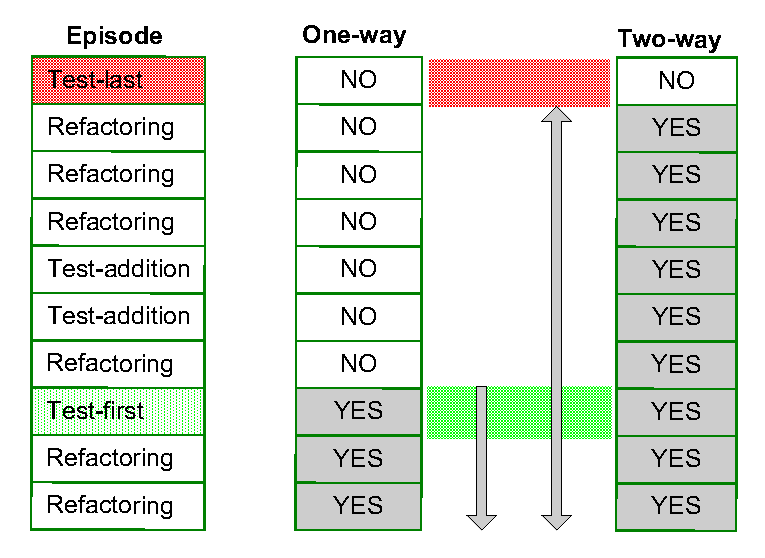
\includegraphics[width=0.8\textwidth]{figs/HeuristicAlgorithms}
  \caption{Heuristic Algorithms of TDD Conformance}
  \label{fig:heuristic}
\end{figure}
There are three lists in Figure \ref{fig:heuristic}. The left-most one is a list of development behaviors recognized by Zorro's inference rules. As their names indicate, the episodes can be ``test-first", ``test-addition", ``refactoring", or ``test-last" etc. The one-way and two-way TDD heuristic algorithms are on the right side of Figure \ref{fig:heuristic}. The one-way algorithm uses look-forward approach to determine whether an episode is TDD conformant, while the two-way heuristic algorithm uses both look-forward and look-backward approaches. Figure \ref{fig:heuristic} indicates this difference using a single-head arrow and a double-head arrow. I implemented these heuristic rules with the support of JESS \cite{Friedman-Hill:03}. Section \ref{sec:Zorro-TDDConformance} in Chapter \ref{ch:Zorro} has a detailed description to this heuristic. Our preliminary work suggests that the two-way heuristic algorithm can understand real world situations better than the one-way algorithm.

\section{Chapter Summary}
This chapter introduced the pilot study, a test to investigate how to validate Zorro using participant observation supported by ESR. The study showed that Zorro's data collection and TDD behaviors inference can be validated by analyzing development videos recorded by ESR. This study also identified several problems that helped to improve Zorro. With these improvements, I conducted an extended classroom case study following the pilot study in my thesis research. 